\documentclass[tikz,border=7pt]{standalone}
\usepackage{amsmath,pgfplots}
\pgfplotsset{compat=1.18}
\definecolor{ink}{HTML}{21352F}\definecolor{teal}{HTML}{087F7B}
\definecolor{gold}{HTML}{C58B2A}\definecolor{blue}{HTML}{4B77A8}\definecolor{rose}{HTML}{B65A62}
\begin{document}
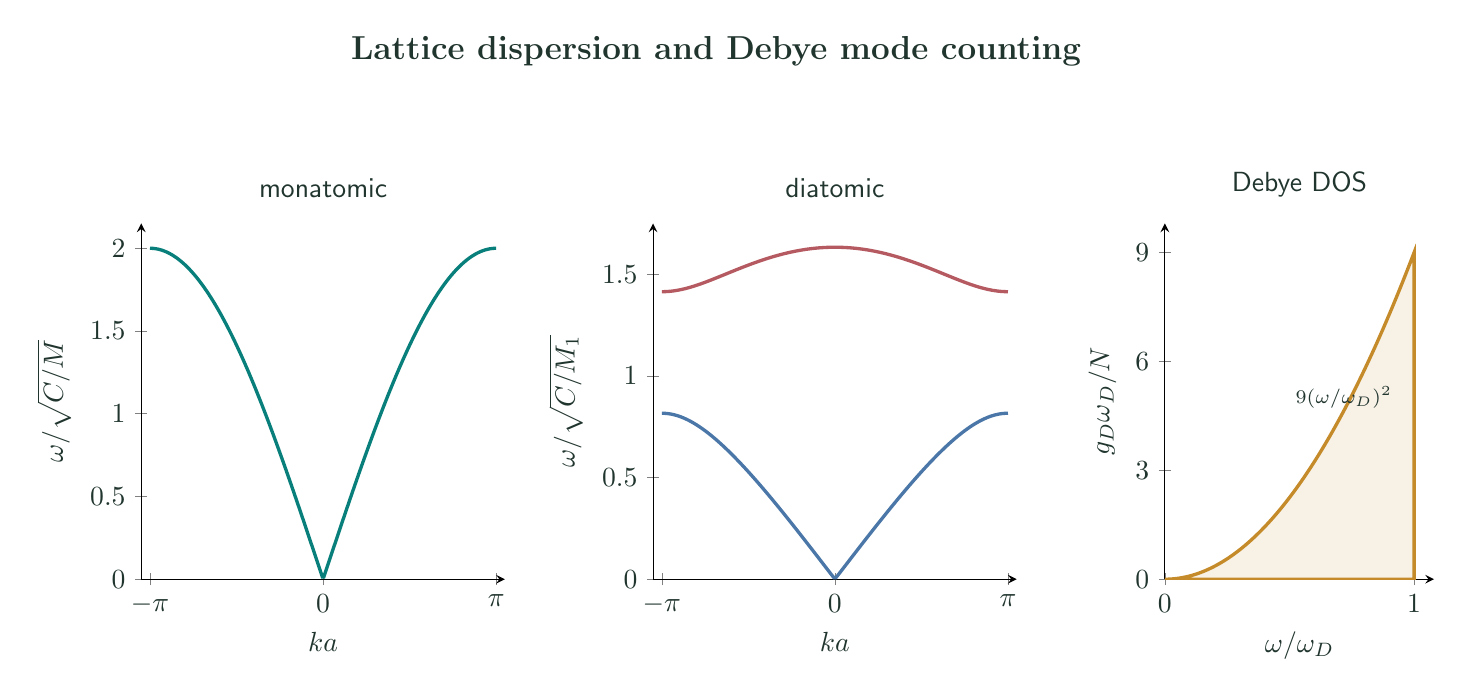
\begin{tikzpicture}[font=\sffamily,text=ink]
\node[font=\bfseries\large] at (0,3.9) {Lattice dispersion and Debye mode counting};
\begin{axis}[at={(-7.3cm,-2.8cm)},anchor=south west,width=6.2cm,height=6.1cm,xmin=-3.3,xmax=3.3,ymin=0,ymax=2.15,
 axis lines=left,xlabel={$ka$},ylabel={$\omega/\sqrt{C/M}$},xtick={-3.1416,0,3.1416},xticklabels={$-\pi$,$0$,$\pi$},title={monatomic}]
 \addplot[teal,very thick,domain=-3.1416:3.1416,samples=220]{2*abs(sin(deg(x)/2))};
\end{axis}
\begin{axis}[at={(-.8cm,-2.8cm)},anchor=south west,width=6.2cm,height=6.1cm,xmin=-3.3,xmax=3.3,ymin=0,ymax=1.75,
 axis lines=left,xlabel={$ka$},ylabel={$\omega/\sqrt{C/M_1}$},xtick={-3.1416,0,3.1416},xticklabels={$-\pi$,$0$,$\pi$},title={diatomic}]
 \addplot[blue,very thick,domain=-3.1416:3.1416,samples=220]{sqrt(1.333333-sqrt(1.777777-1.333333*sin(deg(x)/2)^2))};
 \addplot[rose,very thick,domain=-3.1416:3.1416,samples=220]{sqrt(1.333333+sqrt(1.777777-1.333333*sin(deg(x)/2)^2))};
\end{axis}
\begin{axis}[at={(5.7cm,-2.8cm)},anchor=south west,width=5.0cm,height=6.1cm,xmin=0,xmax=1.08,ymin=0,ymax=9.8,
 axis lines=left,xlabel={$\omega/\omega_D$},ylabel={$g_D\omega_D/N$},xtick={0,1},ytick={0,3,6,9},title={Debye DOS}]
 \addplot[gold,very thick,domain=0:1,samples=140,fill=gold!12]{9*x^2}\closedcycle;
 \node[font=\scriptsize,anchor=east] at (axis cs:.95,5.0) {$9(\omega/\omega_D)^2$};
\end{axis}
\end{tikzpicture}
\end{document}
